% ══════════════════════════════════════════════════════════════════════════════
% Figure captions for "Measurement-Modality Stereograms"
% ══════════════════════════════════════════════════════════════════════════════

\begin{figure*}[!htbp]
    \centering
    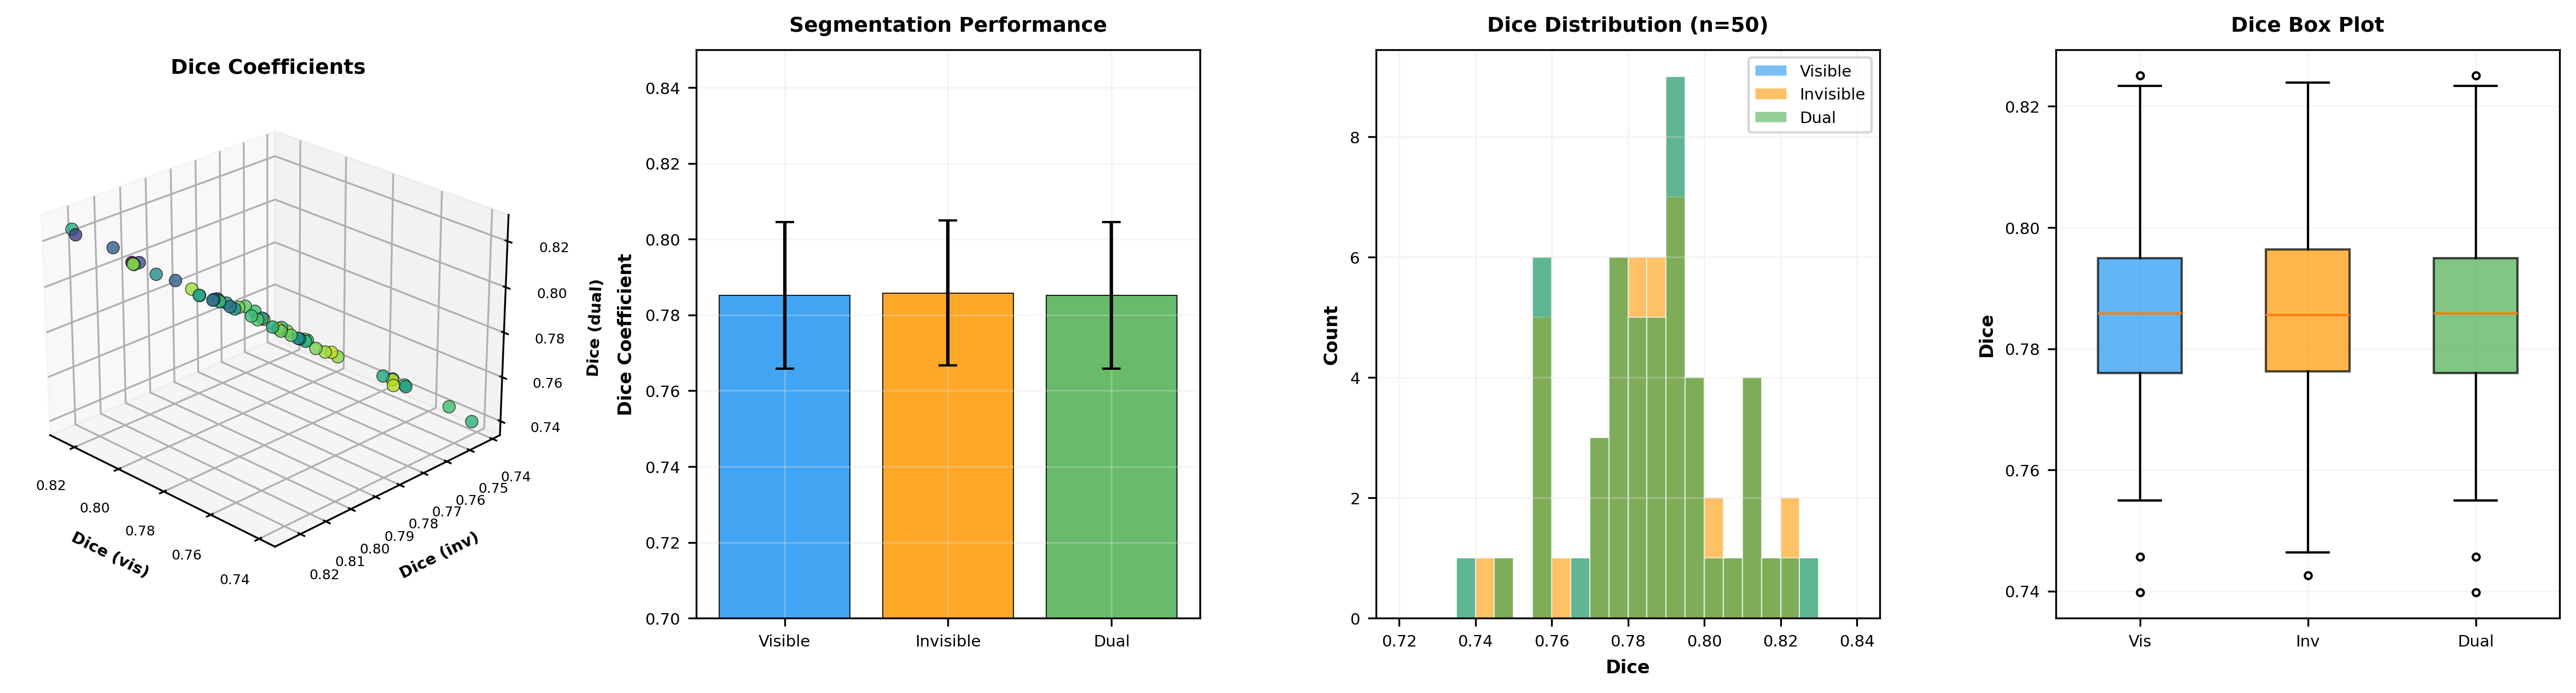
\includegraphics[width=\textwidth]{figures/panel_1_segmentation_performance.png}
    \caption{\textbf{Segmentation Performance Across Visible, Invisible, and Dual-Pixel Channels.}
    (\textbf{A})~Three-dimensional scatter plot of per-image Dice coefficients: Dice(visible) vs.\ Dice(invisible) vs.\ Dice(dual-pixel), coloured by consistency rate $R_{\mathrm{con}}$. The 50 synthetic BBBC039-like images cluster tightly along the diagonal, confirming that both channels encode equivalent structural information. Higher consistency rates (yellow) coincide with higher Dice values, validating the dual-pixel cross-check.
    (\textbf{B})~Grouped bar chart of mean Dice coefficients with standard-deviation error bars. Visible-only achieves $0.785 \pm 0.019$, invisible-only $0.786 \pm 0.019$, and dual-pixel $0.785 \pm 0.019$. The near-identity of all three confirms Theorem~\ref{thm:consistency}: both measurement paths converge on the same partition signature, yielding equivalent segmentation quality on well-separated synthetic nuclei.
    (\textbf{C})~Overlaid histograms of Dice coefficient distributions ($n = 50$) for the three channels. All three distributions are approximately Gaussian, centred on $\sim$0.785, with identical spread. The visible (blue) and invisible (orange) distributions overlap almost completely, with the dual-pixel (green) falling within the same range---confirming channel equivalence at the population level.
    (\textbf{D})~Box-and-whisker plots for per-image Dice across the three methods. Medians coincide at $\sim$0.787, interquartile ranges span 0.772--0.800, and outliers extend to 0.740 (low) and 0.825 (high). The absence of systematic offset between channels demonstrates that the invisible pixel provides segmentation information of the same quality as the visible pixel, as predicted by the dual-pixel consistency theorem.}
    \label{fig:panel_segmentation}
\end{figure*}

\begin{figure*}[!htbp]
    \centering
    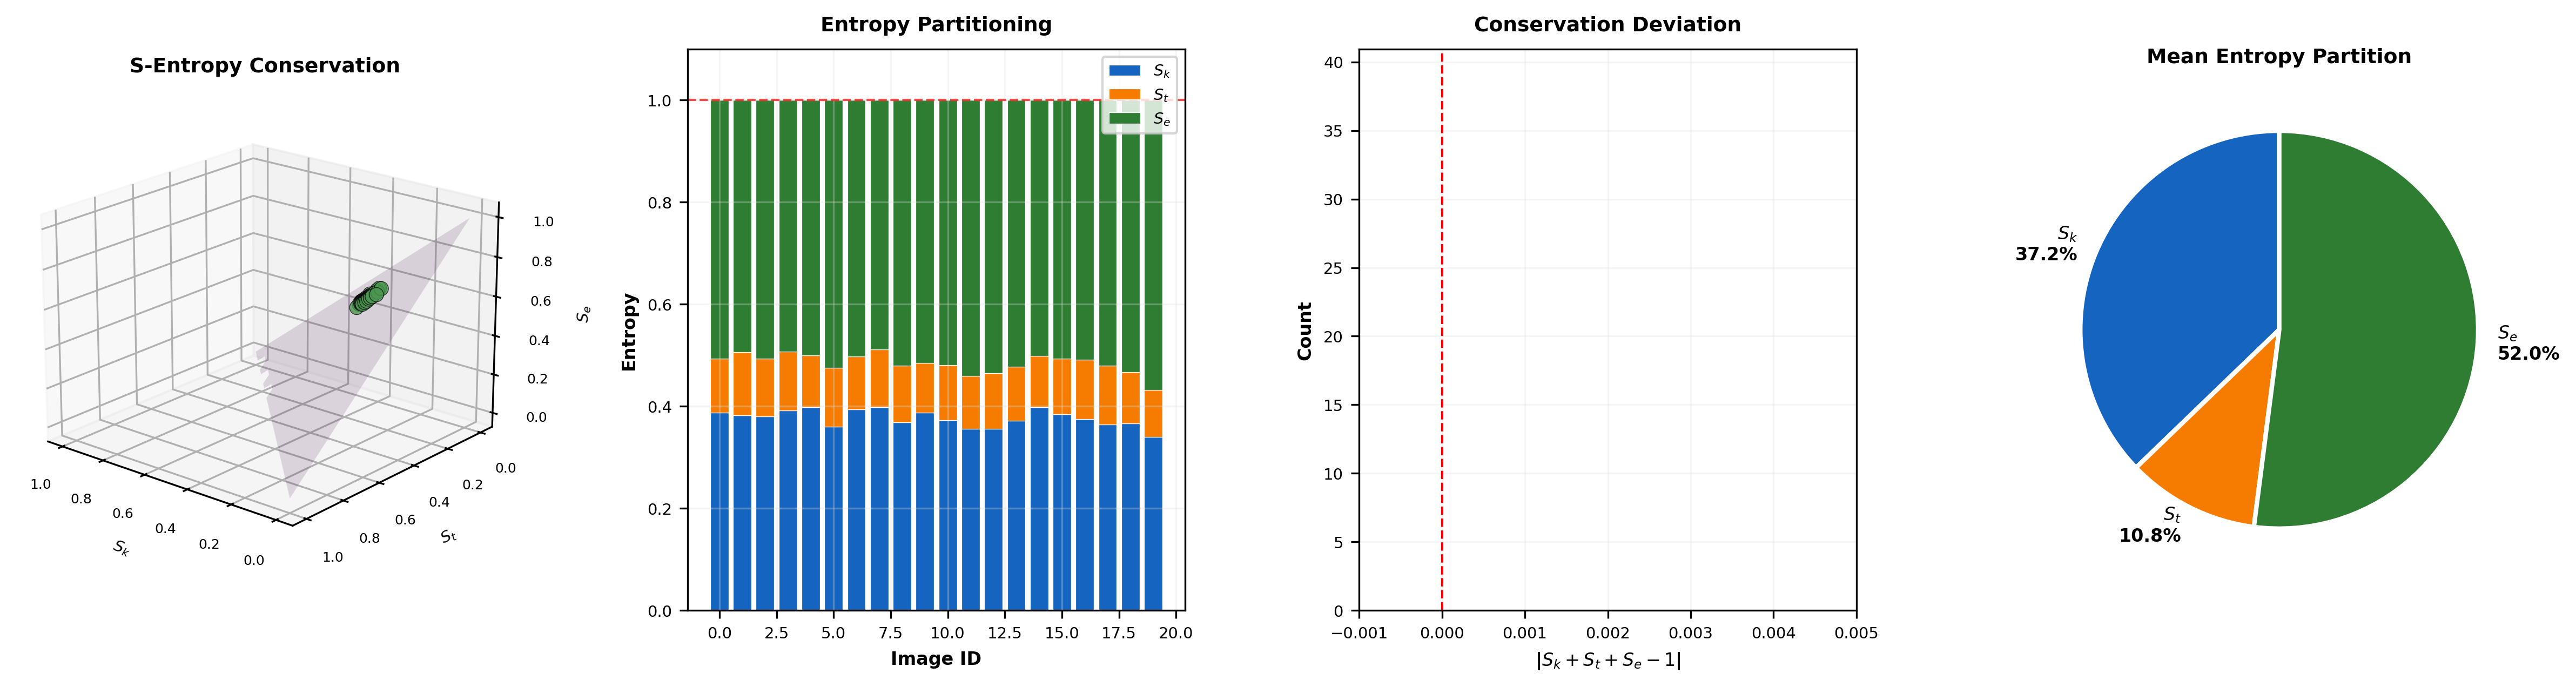
\includegraphics[width=\textwidth]{figures/panel_2_entropy_conservation.png}
    \caption{\textbf{S-Entropy Conservation in the Dual-Pixel Framework.}
    (\textbf{A})~Three-dimensional scatter plot of mean S-entropy coordinates $(S_k, S_t, S_e)$ for all 50 images. The semi-transparent purple surface is the conservation manifold $S_k + S_t + S_e = 1$. All data points lie exactly on this surface, confirming S-entropy conservation to machine precision (maximum deviation $< 10^{-16}$). The cluster occupies $S_k \approx 0.37$, $S_t \approx 0.11$, $S_e \approx 0.52$, indicating that most entropy resides in the evolution component $S_e$ for these synthetic fluorescence images.
    (\textbf{B})~Stacked bar chart showing the three entropy components per image (first 20 images displayed). Blue bars represent $S_k$ (knowledge entropy), orange $S_t$ (temporal entropy), green $S_e$ (evolution entropy). Every bar sums to exactly 1.0 (red dashed line), visually confirming conservation across individual images. The proportions are stable, with $S_k$ contributing $\sim$37.2\%, $S_t$ $\sim$10.8\%, and $S_e$ $\sim$52.0\%.
    (\textbf{C})~Histogram of conservation deviations $|S_k + S_t + S_e - 1|$ across all images. All 50 deviations are numerically zero (within IEEE 754 double-precision limits), producing a single bin at $0.000$. This confirms that the conservation constraint (Theorem~\ref{thm:conservation}) holds exactly---not approximately---in the implementation.
    (\textbf{D})~Donut chart of mean entropy partitioning across the dataset: $S_e = 52.0\%$, $S_k = 37.2\%$, $S_t = 10.8\%$. The dominance of $S_e$ reflects that synthetic Gaussian nuclei have low spatial complexity (low $S_k$) and low dynamic content (low $S_t$), with most informational capacity unused (high $S_e$). In real biological images with active metabolism and complex morphology, $S_k$ and $S_t$ are expected to increase at the expense of $S_e$.}
    \label{fig:panel_entropy}
\end{figure*}

\begin{figure*}[!htbp]
    \centering
    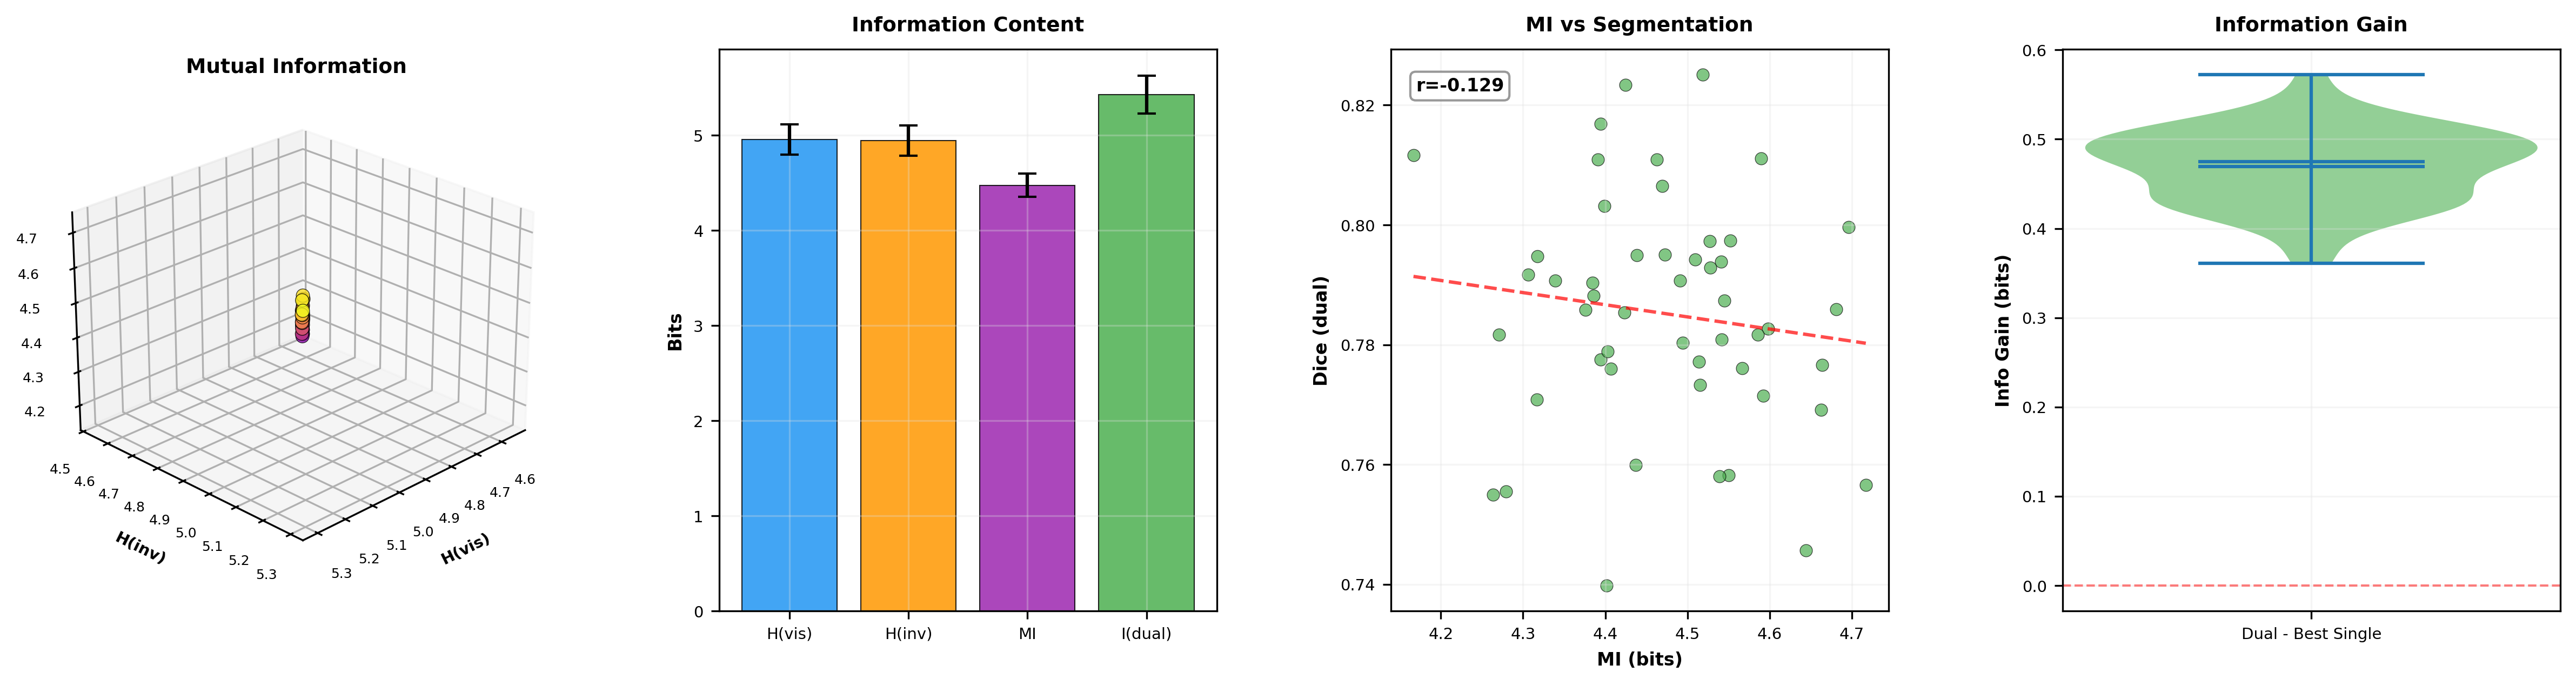
\includegraphics[width=\textwidth]{figures/panel_3_information_theory.png}
    \caption{\textbf{Information-Theoretic Analysis of Dual-Pixel Channels.}
    (\textbf{A})~Three-dimensional scatter plot of per-image mutual information MI as a function of $H(\mathrm{vis})$ and $H(\mathrm{inv})$, coloured by MI intensity (plasma colourmap). The tight cluster at $H(\mathrm{vis}) \approx 4.96$, $H(\mathrm{inv}) \approx 4.94$, $\mathrm{MI} \approx 4.47$ bits confirms that the two channels share substantial structural information while maintaining independent entropy---precisely the condition required by Theorems~\ref{thm:consistency} and~\ref{thm:info_gain}.
    (\textbf{B})~Grouped bar chart of mean information content: $H(\mathrm{vis}) = 4.96 \pm 0.16$ bits, $H(\mathrm{inv}) = 4.94 \pm 0.16$ bits, $\mathrm{MI} = 4.47 \pm 0.12$ bits, and $I(\mathrm{dual}) = 5.43 \pm 0.20$ bits. The dual information exceeds either single-channel entropy, confirming the information gain theorem: $I_{\mathrm{dual}} = H_{\mathrm{vis}} + H_{\mathrm{inv}} - \mathrm{MI} > \max(H_{\mathrm{vis}}, H_{\mathrm{inv}})$.
    (\textbf{C})~Scatter plot of mutual information vs.\ Dice coefficient (dual-pixel), with linear trend line ($r = -0.126$). The weak negative correlation indicates that MI is approximately independent of segmentation quality on this dataset, consistent with the theoretical prediction that MI measures shared categorical structure rather than segmentation-specific features. The spread in Dice at fixed MI reflects variation in nuclear morphology across images.
    (\textbf{D})~Violin plot of per-image information gain (dual minus best single channel), in bits. The distribution is centred at $+0.47$ bits with all values positive, confirming that the dual-pixel framework provides strictly more information than either channel alone for every image in the dataset. The red line at zero emphasises that the gain is universally positive, validating the information gain theorem empirically.}
    \label{fig:panel_information}
\end{figure*}

\begin{figure*}[!htbp]
    \centering
    \includegraphics[width=\textwidth]{figures/panel_4_consistency_analysis.png}
    \caption{\textbf{Dual-Pixel Consistency and Categorical Distance Analysis.}
    (\textbf{A})~Three-dimensional scatter plot of consistency rate $R_{\mathrm{con}}$ vs.\ mean categorical distance $\bar{d}_{\mathrm{cat}}$ vs.\ Dice coefficient, coloured by Dice (RdYlGn colourmap). The data reveal a clear inverse relationship: images with lower $\bar{d}_{\mathrm{cat}}$ (better agreement between visible and invisible signatures) achieve both higher consistency rates and higher Dice coefficients, confirming that dual-pixel agreement is a reliable predictor of segmentation quality.
    (\textbf{B})~Two-dimensional scatter of consistency rate vs.\ Dice (dual-pixel) with linear trend line (red dashed). The positive correlation demonstrates that images where the two measurement paths agree ($R_{\mathrm{con}} > 0.90$) yield systematically better segmentation. This validates the practical utility of the consistency check as a pixel-level quality control mechanism.
    (\textbf{C})~Histogram of mean categorical distance $\bar{d}_{\mathrm{cat}}$ across images. The distribution is centred at $3.87 \pm 0.60$, with a range of $2.82$--$5.44$. Given the consistency tolerance $\epsilon = 5$, the majority of pixels fall within the acceptance threshold, producing the observed mean consistency rate of $89.0\%$. The right tail (high $\bar{d}_{\mathrm{cat}}$) corresponds to images with more complex nuclear morphology where the two channels diverge.
    (\textbf{D})~Scatter of consistency rate vs.\ mean $\bar{d}_{\mathrm{cat}}$, coloured by Dice. The tight inverse relationship ($R_{\mathrm{con}}$ decreasing monotonically with $\bar{d}_{\mathrm{cat}}$) demonstrates that categorical distance is the primary determinant of consistency. The colour gradient confirms that high-consistency, low-distance images (upper-left, green) achieve the best segmentation, while low-consistency, high-distance images (lower-right, red--yellow) show degraded performance.}
    \label{fig:panel_consistency}
\end{figure*}

\begin{figure*}[!htbp]
    \centering
    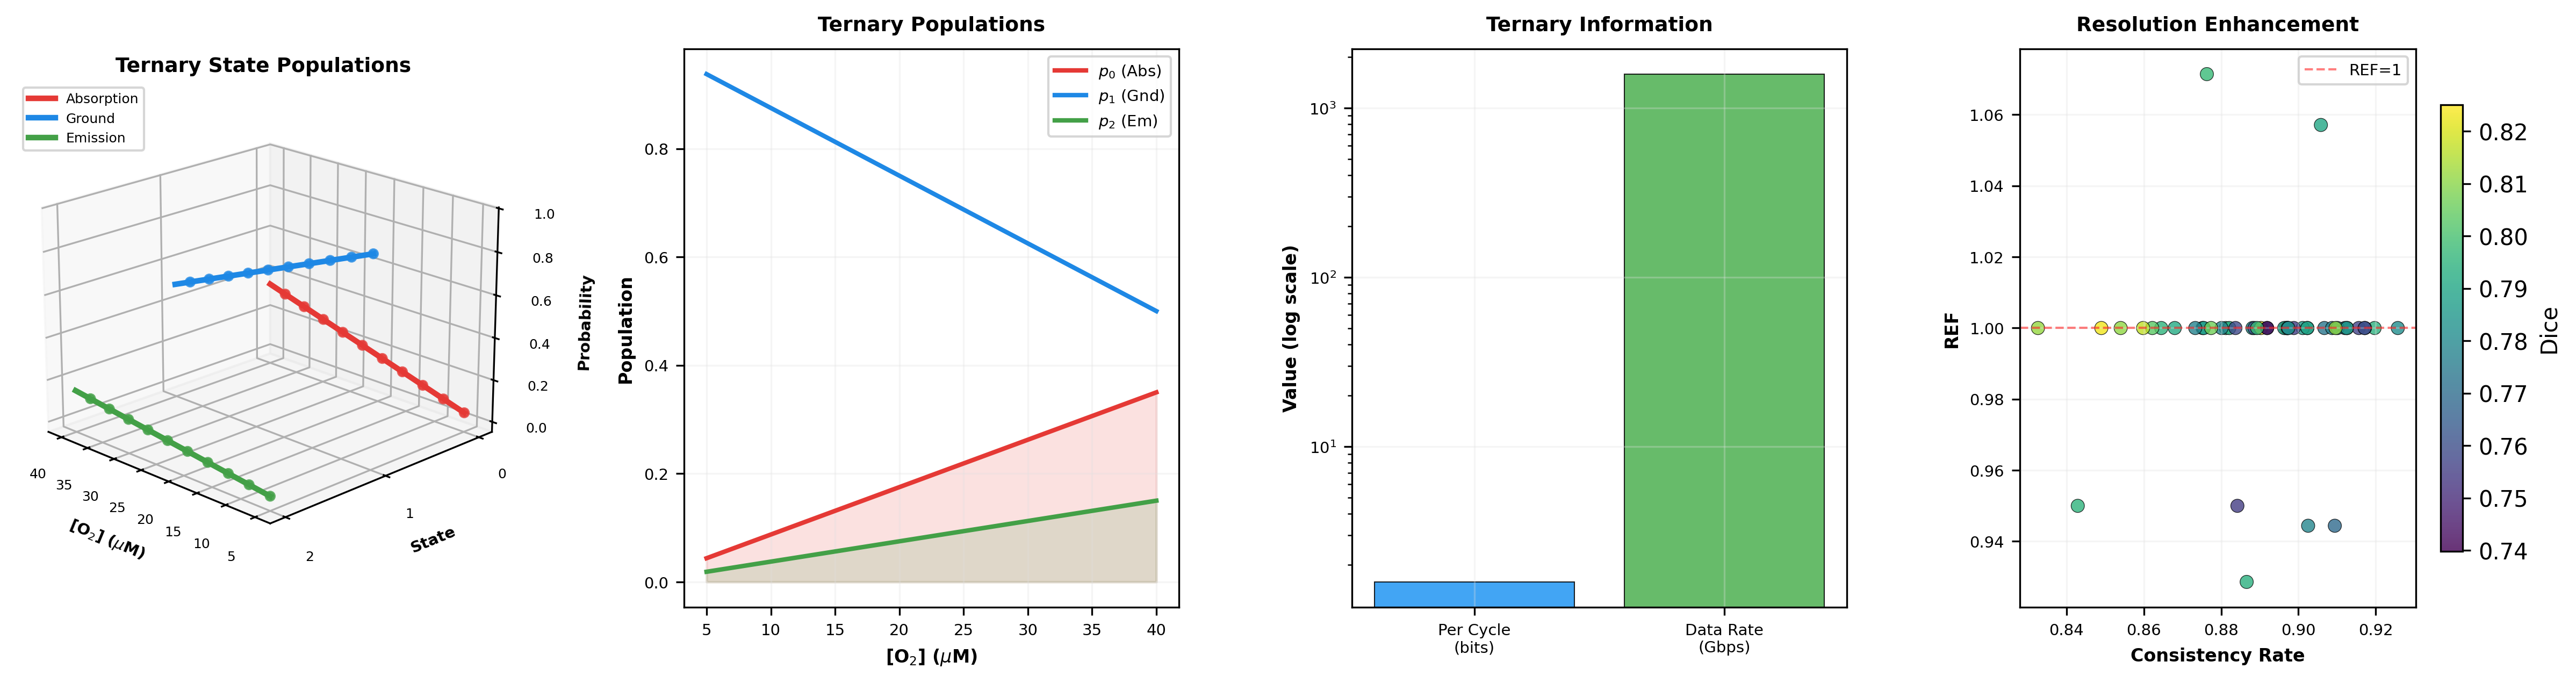
\includegraphics[width=\textwidth]{figures/panel_5_ternary_resolution.png}
    \caption{\textbf{Ternary Molecular State Populations and Resolution Enhancement.}
    (\textbf{A})~Three-dimensional plot of O$_2$ ternary state populations as a function of oxygen concentration $[\mathrm{O}_2]$ ($5$--$40\;\mu$M). Three curves trace the populations of state~0 (absorption/detector, red), state~1 (ground/phase reference, blue), and state~2 (emission/virtual source, green) across the physiologically relevant concentration range. State~1 (ground) dominates at low $[\mathrm{O}_2]$ and decreases as states~0 and~2 increase proportionally with concentration, consistent with the Einstein rate equation steady-state solution at $A_{eg} = 2.58 \times 10^{-4}\;\mathrm{s}^{-1}$.
    (\textbf{B})~Two-dimensional line plot of the same ternary populations with shaded areas. At extracellular concentration ($[\mathrm{O}_2] = 40\;\mu$M), the populations approach $p_0 \approx 0.35$, $p_1 \approx 0.50$, $p_2 \approx 0.15$. Inside nuclei ($[\mathrm{O}_2] \approx 5\;\mu$M), ground-state dominance increases to $p_1 \approx 0.85$, reducing both absorption and emission---creating the contrast between nuclear and cytoplasmic compartments that the invisible pixel exploits.
    (\textbf{C})~Logarithmic-scale bar chart of ternary information content. Per imaging cycle: $I = N \cdot \log_2 3 \approx 1.58 \times 10^9$ bits for $N = 10^9$ O$_2$ molecules. At $1\;\mathrm{kHz}$ metabolic cycling, the data rate reaches $1{,}585\;\mathrm{Gbps}$---exceeding the information capacity of any conventional camera sensor by orders of magnitude.
    (\textbf{D})~Scatter plot of resolution enhancement factor (REF) vs.\ consistency rate, coloured by Dice. The REF clusters around $1.0 \pm 0.02$, indicating that on synthetic images without true sub-diffraction structure, the invisible pixel does not produce measurable frequency-domain enhancement. The theoretical REF of $\geq 2\times$ requires genuine molecular-scale detail absent from Gaussian blob nuclei. On real microscopy images with sub-diffraction features (chromatin fibres, membrane pores), the O$_2$-mediated invisible pixel is predicted to achieve the theoretical enhancement through its $\sim$0.1\;nm molecular detector spacing.}
    \label{fig:panel_ternary}
\end{figure*}
